\subsection{Density Visualization}
\label{app:density_visualization}

Figure~\ref{fig:appendix_density_visualization} compares point allocation
for the eight showcase cases at a $37.5\%$ budget. Within each spatial bin
$B$, we display the retained fraction
$n_{\mathrm{selected}}(B)/n_{\mathrm{reference}}(B)$ on a common scale.
Uniform gives approximately constant retention, while the adaptive policies
redistribute points across the domain.

\begin{figure}[!ht]
    \centering
    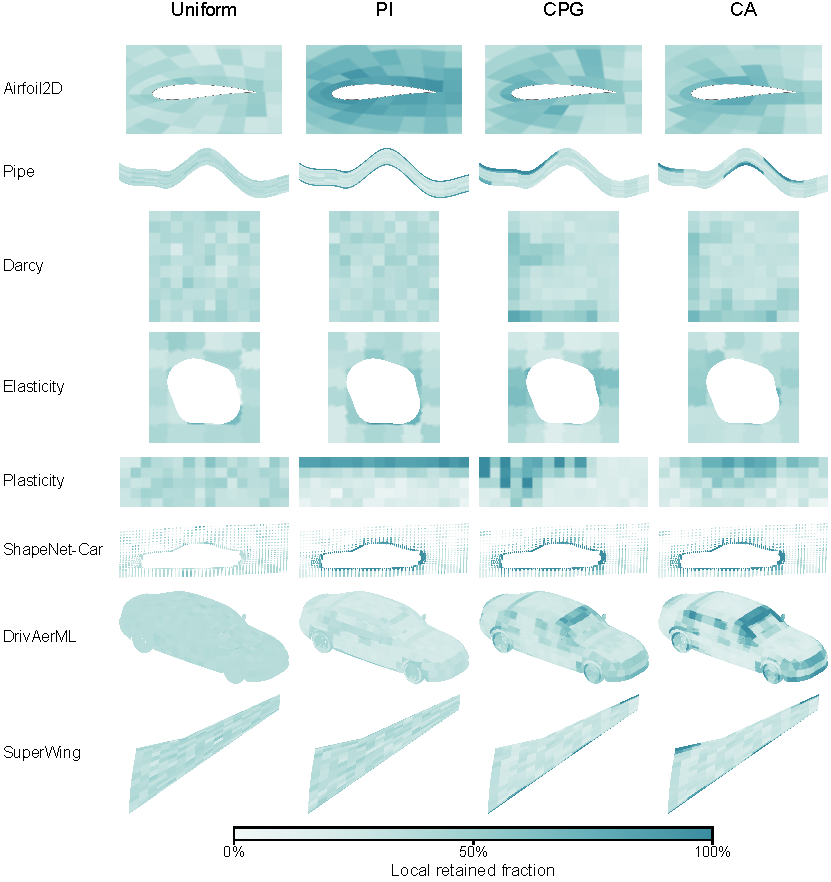
\includegraphics[width=\linewidth,height=.74\textheight,keepaspectratio]{figures/appendix/density_visualization.pdf}
    \caption{\textbf{Local sampling retention.} Rows show the same eight
    cases used in Appendix~\ref{app:field_visualizations}, with sampling
    seed zero. Darker colors indicate a larger fraction of reference points
    retained within each bin. All methods share the same color scale.}
    \label{fig:appendix_density_visualization}
\end{figure}
